\documentclass[12pt,a4paper,titlepage,openany]{report}
\usepackage{zakljucna_FAMNIT_1_stopnja_MA_MEF_EN_2016}
\usepackage{subcaption}
\usepackage{float}
\usepackage{graphicx}
\graphicspath{ {./images/} }


% Head of document:

\fancyhf{}
\lhead[]{{\fontsize{9.3}{12}\selectfont
Convolutional neural network for eyeblink artifact detection in EEG data.\\
\noindent Univerza na Primorskem, Fakulteta za matematiko, naravoslovje in informacijske tehnologije, 2025}}
\chead[]{\fancyplain{}{}}
\rhead[]{\fancyplain{\thepage}
{\thepage}}
\cfoot[]{\fancyplain{}{}}
\lfoot[]{\fancyplain{}{}}
\rfoot[]{\fancyplain{}{}}
\normalsize

%%%%%%%%%%%%%%%%%%%%%%%%% BEGINNING OF DOCUMENT %%%%%%%%%%%%%%%%%%%%%%%%%%%%%%%%%%%%%%%%%%5

%%%%%%%%%%%%%%%%%%%%%%%%% Title page %%%%%%%%%%%%%%%%%%%%%%%%%


\begin{document}
\pagenumbering{Roman}
\pagestyle{empty}
\begin{center}
\noindent \large UNIVERZA NA PRIMORSKEM\\
\large FAKULTETA ZA MATEMATIKO, NARAVOSLOVJE IN\\
INFORMACIJSKE TEHNOLOGIJE


\normalsize
\vspace{5.5cm}
Zaklju\v cna naloga\\
(Final project paper)\\
\textbf{\large Naslov zaklju\v cne naloge}\\
\normalsize
(Convolutional neural network for eyeblink artifact detection in EEG data)\\
\end{center}

\begin{flushleft}
\vspace{5cm}
\noindent Ime in priimek: Marko Janković
% add your first name and last name in the line above
\\
\noindent \v Studijski program: (name of the study program, in Slovene)
% add your study program in the line above
\\
\noindent Mentor: (with all titles, in Slovene)
% add the academic title, first name, and last name of your mentor in the line above
\\
\noindent Somentor: (with all titles, in Slovene)
% if you have a co-mentor, add his/her academic title, first name, and last name in the line above
% if you do not have a co-mentor, delete the line above and the line below
\\
\end{flushleft}

\vspace{4cm}
\begin{center}
\large \textbf{Koper, mesec 2025}
% add the month and year of submission of your final project paper
\end{center}
\newpage

\pagestyle{fancy}
%%%%%%%%%%%%%%%%%%%%%%%%%%%%%%% Key words documentation (Slovene and English) %%%%%%%%%%%

\section*{Klju\v cna dokumentacijska informacija}

\medskip
\begin{center}
\fbox{\parbox{\linewidth}{
\vspace{0.2cm}
\noindent
Ime in PRIIMEK: Marko Janković \vspace{0.5cm}\\
Naslov zaklju\v cne naloge:\vspace{0.5cm}\\
Kraj: Koper\vspace{0.5cm}\\
Leto: 2025 \vspace{0.5cm}\\
\v Stevilo listov: \hspace{2cm} \v Stevilo slik: \hspace{2.6cm} \v Stevilo tabel:\hspace{2cm}\vspace{0.5cm}\\
\v Stevilo prilog: \hspace{1.9cm} \v Stevilo strani prilog: \hspace{1cm} \v Stevilo referenc:\vspace{0.5cm}\\
Mentor:\vspace{0.5cm}\\
Somentor:\vspace{0.5cm}\\
Klju\v cne besede:\vspace{0.5cm}\\
{\bf Izvle\v cek:}\\
Izvle\v cek predstavlja kratek, a jedrnat prikaz vsebine naloge. V najve\v c 250 besedah nakažemo problem, metode, rezultate, klju\v cne ugotovitve in njihov pomen.
\vspace{0.2cm}
}}
\end{center}

\newpage

\section*{Key words documentation}

\medskip

\begin{center}
\fbox{\parbox{\linewidth}{
\vspace{0.2cm}
\noindent
Name and SURNAME: Marko Janković\vspace{0.5cm}\\
Title of final project paper: Convolutional neural network for eyeblink artifact detection in EEG data\vspace{0.5cm}\\
Place: Koper \vspace{0.5cm}\\
Year: 2025\vspace{0.5cm}\\
Number of pages:\hspace{1.6cm} Number of figures:\hspace{2.2cm} Number of tables:\vspace{0.5cm}\\
Number of appendices:\hspace{0.6cm} Number of appendix pages:\hspace{0.8cm}Number of references:\vspace{0.5cm}\\
Mentor: title~First Name~Last Name, PhD\vspace{0.5cm}\\
% for : "title" write one of the following:
% Assist.~Prof.~(if the title is "docent"),
% Assoc.~Prof.~(if the title is "izredni profesor"),
% Prof.~(if the title is "profesor")
Co-Mentor:\vspace{0.5cm}\\
Keywords:\vspace{0.5cm}\\
{\bf Abstract:}
\vspace{0.2cm}
}}
\end{center}




%%%%%%%%%%%%%%%%%%%%%%%%%%%%%%% Acknowledgement %%%%%%%%%%%%%%%%%%%%%%%%%%%%%%%%%%%%%

\newpage
\section*{Acknowledgement}

Here we thank all involved with our final project paper, that is, persons or institutions that helped us in our work and/or made it possible.
We can also thank the mentor and the co-mentor (if there is one).

%%%%%%%%%%%%%%%%%%%%%%%%%%%%% Table of contents, list of figures, etc. %%%%%%%%%%%%%%%%%%%%%%%%%%%%%%
\newpage

\tableofcontents
\addtocontents{toc}{\protect\thispagestyle{fancy}}
% if there are no tables in your final project paper, delete the following three lines
\newpage
\listoftables
\addtocontents{lot}{\protect\thispagestyle{fancy}}
% if there are no figures in your final project paper, delete the following three lines
\newpage
\listoffigures
\addtocontents{lof}{\protect\thispagestyle{fancy}}
\newpage

\chapter*{List of Abbreviations}
\thispagestyle{fancyplain}
\begin{longtable}{@{}p{2cm}@{}p{\dimexpr\textwidth-2cm\relax}@{}}
\nomenclature{{\it EEG}}{ Electroencephalogram}
\nomenclature{{\it ICA}}{ Independent Component Analysis}
\nomenclature{{\it CNN}}{ Convolutional Neural Network}
\nomenclature{{\it fMRI}}{Functional magnetic resonance imaging}
\nomenclature{{\it NIRS}}{Near-infrared spectroscopy}
\nomenclature{{\it NLP}}{Natural language processing}
\nomenclature{{\it RNN}}{Recurrent neural network}
\nomenclature{{\it LSTM}}{Long short-term memory}
\nomenclature{{\it GRU}}{Gated recurrent unit}
\nomenclature{{\it TCN}}{Temporal Convolutional Network}
\nomenclature{{\it PCA}}{Principal Component Analysis}
\nomenclature{{\it FCN}}{Fully-convolutional network}
\end{longtable}
\newpage

\normalsize

%%%%%%%%%%%%%%%%%%%%%%%%%%%%%%%%%% Chapters: %%%%%%%%%%%%%%%%%%%%%%%%%%%%%%%%%%%%%

% Hint: You might find it convenient to keep the contents of separate chapters in separate files, each in their own
% .tex file. They all have to be stored in the same folder as the main file. Each chapter is included with the \include command.
% Example: we can insert FirstChapter.tex and SecondChapter.tex as follows:
% \include{FirstChapter}
% \include{SecondChapter}

%%%%%%%%%%%%%%%%%%%%%%%%%%%%%%%%%% Chapter 1: Introduction %%%%%%%%%%%%%%%%%%%%%%%%%%%%%%%%%%%%%


\chapter{Introduction}
\thispagestyle{fancy}
\pagenumbering{arabic}

Electroencephalogram (EEG) is a non-invasive neuroimaging technique that involves the placement of electrodes on the scalp to record the electrical activity of the brain\cite{islam2023}. This enables researchers to measure and analyze the electrical signals generated by the brain. These signals offer valuable information on the functioning mechanisms of the brain, covering the identification of various neurological disorders and the exploration of cognitive processes such as perception, attention, and memory.
However, EEG signals are prone to various artifacts, one of the most common being eye blinks, which for adults typically occur 15-20 times per minute. Eye closure changes brain activity, so eye blink tracking of subjects undergoing EEG analysis is relevant to identify when a subject blinks, falls asleep, or keeps their eyes closed. 
Eye blink and muscle movement artifacts are usually unwanted signals in the brain that can contaminate EEG data significantly and affect the accuracy of subsequent analysis of brain activity that is being measured with an electroencephalogram (EEG). 
Traditional methods for detecting and removing eye blink artifacts involve manual inspection, filtering, or statistical techniques like Independent Component Analysis (ICA). While these methods can work, they are very time-consuming and prone to human error, especially in real-time applications. They also fail to capture the complex spatial and temporal relationships in EEG data, hence they vary for different subjects and recording conditions.

\section{Purpose of the thesis}

In recent years Convolutional Neural Networks (CNN) have shown to be very effective in various domains as they can learn hierarchical features from raw data. 
This thesis proposes a CNN-based approach to detect signals in EEG data automatically, by demonstrating this ability on detection of eye blink artifacts. 
The aim is to design a model to detect pretrained events through EEG analysis and with that prove that neural networks can be used to enhance EEG recordings.

%%%%%%%%%%%%%%%%%%%%%%%%%%%%%%%%%% Chapter 2: Background and context %%%%%%%%%%%%%%%%%%%%%%%%%%%%%%%%%%%%%

\chapter{Background and context}
\thispagestyle{fancy}

In this section we lay the ground work for the thesis by explaining some of the core components that will be used in proving our thesis.

\section{Electroencephalography (EEG)}

Electroencephalography (EEG) \cite{wikipediaEEG} is the measurement of the electric potentials on the scalp surface generated (in part) by neural activity originating from the brain. 
The sensitivity of EEG to changes in brain activity on such a millisecond time scale is the major advantage of EEG over other brain imaging modalities such as functional magnetic resonance imaging (fMRI) or near-infrared spectroscopy (NIRS) that operate on time scales in the seconds to minutes range. 
Over the past 100 years, neuroscientists and clinical neurologists have made use of EEG to obtain insight into cognitive or clinical disease state by applying a variety of signal processing and statistical analyses to EEG time series. 
More recently there has been growing interest in making use of statistical modeling of EEG signals to directly control physical devices in Brain-Computer Interfaces\cite{nunez2016}.

Brain waves have been categorized into four basic groups \cite{teplan2002} as we can see in Figure \ref{fig:brain-waves}: 
\begin{itemize}
    \item Beta (\textgreater13 Hz), which is usual working rhythm
    \item Alpha (8-13 Hz), appears  during  relaxation  without attention and concentration.
    \item Theta (4-8 Hz), theta waves in adults while awake is abnormal, they are generated by access to unconscious material, deep inspiration and meditation 
    \item Delta (0.5-4 Hz), usually happens during deep sleep\cite{khalifa2012}.
\end{itemize}

\begin{figure}[H]
     \centering
     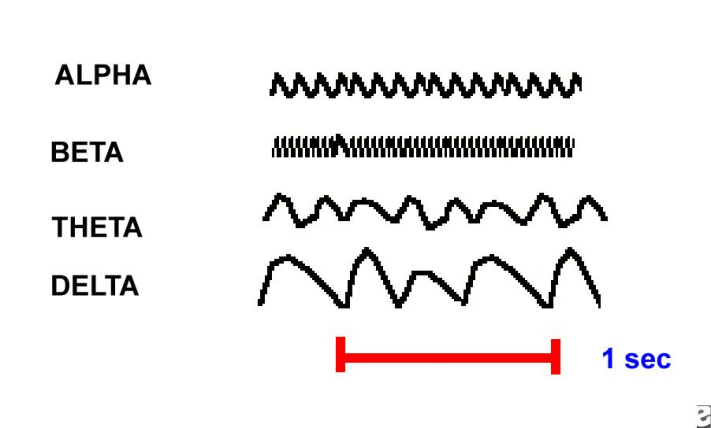
\includegraphics[width=1\linewidth]{./misc/waves.png}
     \caption{Samples of EEG demonstrating the major frequency bands that are presented at various stages of cognitive activity\cite{khalifa2012}.}
     \label{fig:brain-waves}
\end{figure}

For location electrodes the 10-20 system \cite{wikipedia1020} has been used, which is the internationally recognized method to describe and apply the location of scalp electrodes in the context of an EEG exam. The system is based on the relationship between the location of an electrode and the underlying area of the brain, specifically the cerebral cortex.

As we can see from Figure \ref{fig:channel-locations}, we have 32 electrodes placed on the head, and each electrode placement site has a letter to identify the lobe, or area of the brain it is reading from: pre-frontal (Fp), frontal (F), temporal (T), parietal (P), occipital (O), and central (C). There are also (Z) sites: A "Z" (zero) refers to an electrode placed on the midline sagittal plane of the skull, (FpZ, Fz, Cz, Oz) and is present mostly for reference/measurement points. Even-numbered electrodes (2,4,6,8) refer to electrode placement on the right side of the head, whereas odd numbers (1,3,5,7) refer to those on the left.

\begin{figure}[H]
     \centering
     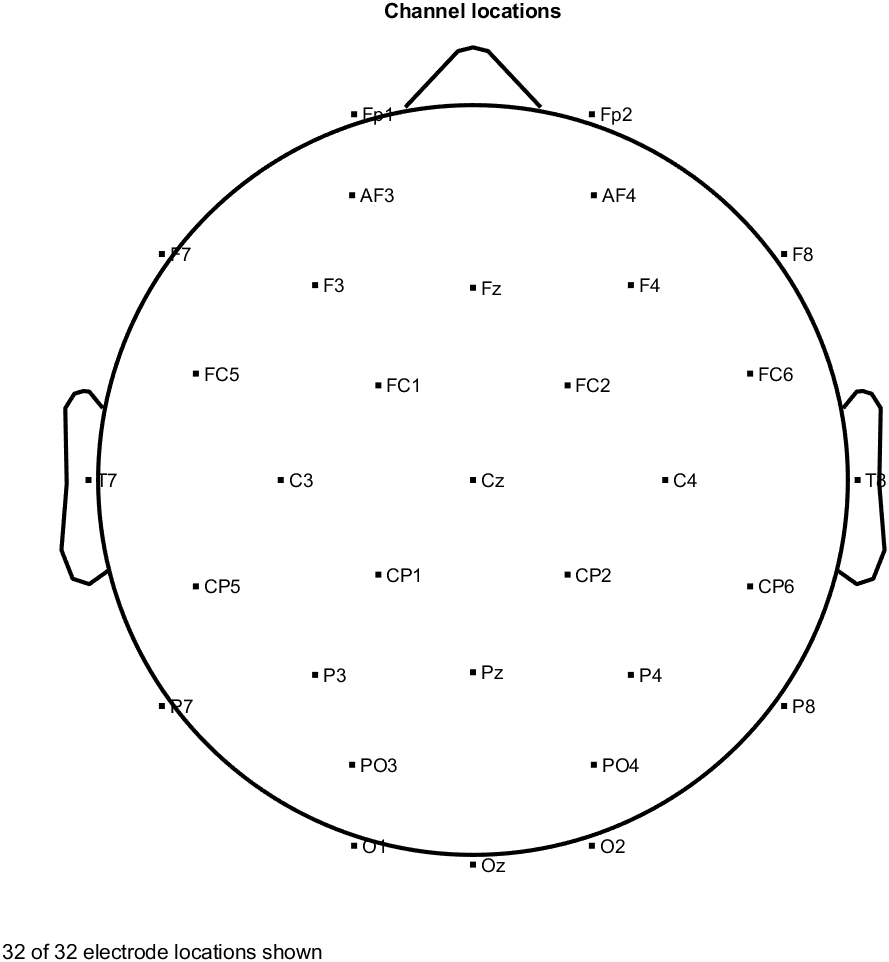
\includegraphics[width=0.7\linewidth]{./misc/Channel locations.png}
     \caption{Channel locations}
     \label{fig:channel-locations}
\end{figure}

\section{Neural Networks}

Convolutional networks have been applied to sequences for decades. They were used prominently for speech recognition in the 80s and 90s. 
ConvNets were subsequently applied to natural language processing (NLP) tasks such as part-of-speech tagging and semantic role labelling. 
More recently, convolutional networks were applied to sentence classification and document classification. 
Recurrent networks are dedicated sequence models that maintain a vector of hidden activations that are propagated through time. 
This family of architectures has gained tremendous popularity due to prominent applications to language modeling and machine translation. 
The intuitive appeal of recurrent modeling is that the hidden state can act as a representation of everything that has been seen so far in the sequence. 
Basic recurrent neural network (RNN) architectures are notoriously difficult to train and more elaborate architectures are commonly used instead, such as the Long short-term memory (LSTM) and the Gated recurrent unit (GRU). 
Many other architectural innovations and training techniques for recurrent networks have been introduced and continue to be actively explored.
Other recent works have aimed to combine aspects of RNN and CNN architectures. This includes the Convolutional LSTM, which replaces the fully-connected layers in an LSTM with convolutional layers to allow for additional structure in the recurrent layers; the Quasi-RNN model that interleaves convolutional layers with simple recurrent layers; and the dilated RNN, which adds dilations to recurrent architectures.\\

First, we describe a generic architecture for convolutional sequence prediction. 
The aim is to distill the best practices in convolutional network design into a simple architecture that can serve as a convenient but powerful starting point. 
The presented architecture is referred to as a temporal convolutional network (TCN), emphasizing that this term serves not as a label for a truly new architecture, but as a simple descriptive term for a family of architectures. 
The distinguishing characteristics of TCNs are: 
\begin{enumerate}
     \item the convolutions in the architecture are causal, meaning that there is no information “leakage” from future to past; 
     \item the architecture can take a sequence of any length and map it to an output sequence of the same length, just as with an RNN. 
\end{enumerate}   
Beyond this, it is emphasized how to build very long effective history sizes (i.e., the ability for the networks to look very far into the past to make a prediction) using a combination of very deep networks (augmented with residual layers) and dilated convolutions. The architecture is informed by recent convolutional architectures for sequential data, but is distinct from all of them and was designed from first principles to combine simplicity, autoregressive prediction, and very long memory. For example, the TCN is much simpler than WaveNet (no skip connections across layers, conditioning, context stacking, or gated activations). 
Compared to the other language modeling architectures, TCNs do not use gating mechanisms and have much longer memory\cite{bai2018}.

\section{ICA analysis}

ICA was firstly created for dealing with the cocktail party problem, upon which you attempt to isolate a pertinent conversation from the noise of other conversations in a cocktail party. Applying the ICA to the EEG data involves the decomposition of EEG time series data into a set of components. More specifically, EEG data are transformed to a collection of simultaneously recorded outputs of spatial filters applied to the whole multi-channel data, instead of a collection of simultaneously recorded single-channel data records. Thus, ICA is also a source separation technique that attempts to identify independent sources of variance in the EEG data. 
In the original EEG data collected at single channels, each row of the recording data matrix represents the time course of summed in voltage differences between the respective channel and the references channels. 
After ICA decomposition, each row of the transformed data matrix represents the time course of the activity of one independent component that is spatially filtered from the channel data. 
The outputs of ICA procedure are statistically independent component (IC) waveforms, as well as matrix that transforms EEG data to IC data, and its inverse matrix to transform IC data back to EEG data. 
These outputs provide information about an IC’s temporal and spatial properties. Concerning that ICA assumes an instantaneous relationship (e.g., common volume conduction) and that any relationship between EEG and EMG signals should involve propagation delays, it is recommended to only select EEG channels for ICA decomposition\cite{makkar2023}.

\begin{figure}[H]
     \centering
     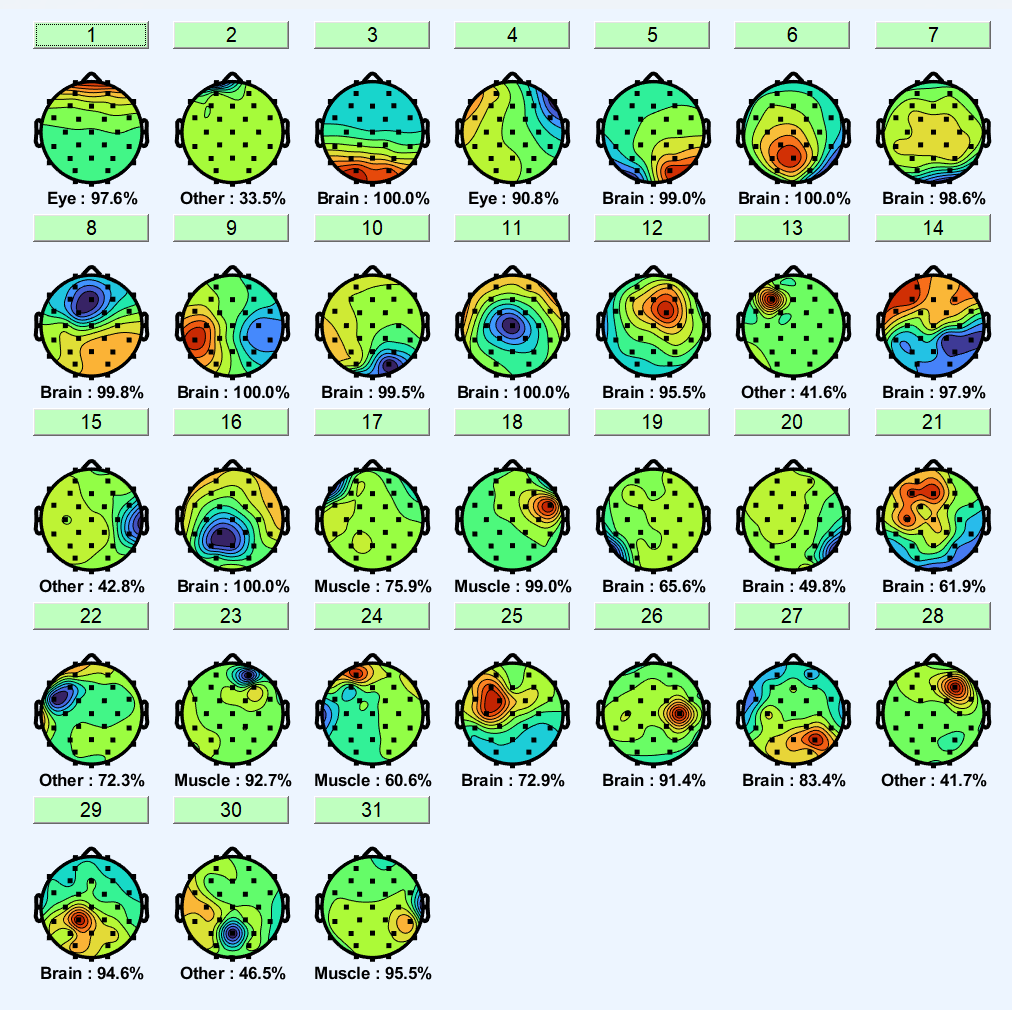
\includegraphics[width=0.8\linewidth]{./misc/Component Properties.png}
     \caption{ICA labeled component properties}
     \label{fig:component-properties-ICA}
\end{figure}


%%%%%%%%%%%%%%%%%%%%%%%%%%%%%%%%%% Chapter 3: Methodology %%%%%%%%%%%%%%%%%%%%%%%%%%%%%%%%%%%%%


\chapter{Methodology}
\thispagestyle{fancy}

In this section, the proposed methodology is described stepwise. First, a description of the data is given, and then the data pre-processing is explained, followed by the architecture of the model.

\section{Dataset}

We obtained and used dataset from the research about the complexity of caffeine's effects on regular coffee consumers\cite{lesar2025}.

\subsection{Dataset description}

This dataset examines the effects of caffeine on brain stimulation and consists of EEG recordings of two categories of participants: the first group which had an intake of regular coffee, and the other which had decaffeinated coffee. 
The primary difference between the two types of participants was the drinks and hence caffeine content. 
Participants from both groups were given the chance to add different amounts of sugar to their drinks, which causes an issue with the data but this is not the concern of this analysis.
The dataset contains three subsets, that is, three different human subjects and data from their EEG measurements.

In relation to our project, this dataset will be used for dealing with artifact identification and detection in EEG data, and while the original research was focused on caffeine stimulation of the brain, we are interested only in artifacts present in EEG signals, such as blinking, movements of muscles, and other activities nearby that interfere with the EEG readings.

\subsection{Data preprocessing}

Although EEG recordings tend to contain noise and artifacts, such as blinking or movement of the eyes, EEG signals measured from the scalp do not necessarily accurately represent signals originating from the brain. 
Therefore, it is very essential to apply preprocessing and denoising to the recorded EEG data. 
Generally, preprocessing steps include the transformations or reorganizations of the recorded EEG data by removing bad or artifact-ridden data without changing clean data (transformation) and segmenting continuous raw signals without change of the data (reorganizations).

Our data preprocessing comes in four steps:
\begin{enumerate}
    \item Filter 1 to 50Hz:
    
    We apply a bandpass filter to the EEG data, keeping frequencies between 1 Hz (lower limit) and 50 Hz (upper limit).

    1 Hz: This high-pass filter removes very slow components (below 1 Hz) that may correspond to artifacts like slow drifts in signals.

    50 Hz: This low-pass filter removes fast components above 50 Hz, such as muscle artifacts and electrical noise.

    \item Cutaway first 1000 samples

    We remove the first 1000 samples, which might correspond to initial noise or artifacts at the start of the recording. 

    \item Re-reference to average

    This step re-references the EEG signals by subtracting the average of all electrodes from each electrode. This is commonly done to minimize noise and make the signals more comparable across channels.

    The assumption of average reference is: the sum of the electric field values recorded at all scalp electrodes (sufficiently dense and evenly distributed) is always 0, and the current passing through the base of the skull to the neck and body is negligible. 
    Since our EEG recording system has enough even channels using average reference makes sense as the overall activity averages to 0.

    \item Resample from 600 to 300 Hz

    We resample the data from a sampling rate of 600 Hz to 300 Hz. Resampling reduces the data size while retaining enough frequency resolution for EEG analysis.

\end{enumerate}

\section{ICA label based artifact detection}

The EEG data recorded from scalp electrodes can be considered summations of real EEG signals and artifacts, which are independent of each other. ICA is therefore potentially a useful methodology to separate artifacts from EEG signals. To removal artifacts embedded in EEG recordings, the computed ICs are firstly classified as either artefactual or neural related components. If detected and flagged as artifact-related ICs, they can be subtracted from the recorded data, and the remaining data can be remixed. In the artifact correction, ICA is used to separate components in order to identify artifacts relevant with eye movements or heartbeats. 
These relevant ICs have characteristic shapes (topographies, time courses, and frequency spectra) and can often be identified automatically. 
That is, artifact-relevant components generally can be identified according to the topographies, across-trial temporal distributions, and frequency distributions of the components. 

Abnormal topographies can be appeared as (1) power concentrated only in the frontal lobe in topography (ocular artifacts); (2) discontinued topography (noise artifacts); and (3) topography constrained within single electrode (electrode artifacts). 
Abnormal across-trial temporal distributions can be appeared as (1) inconsistent between epochs (without obvious peaks in average waveforms); (2) periodic waveform (power line interference); and (3) noisy pattern (similar to Gaussian noise). 
In addition, the frequency of artifact relevant components is in higher-frequency band (e.g., \textgreater 30 Hz), while the frequency content of neural signals is in lower-frequency band (e.g., 5–20 Hz). 
Particularly, for components relevant with blink artifacts (as shown in Fig. \ref{fig:ICA}), they have an anterior distribution, and their time courses are largely flat with occasional very high-amplitude spikes indicating artifacts of the eye muscles as they close and open.

\begin{figure}[H]
     \centering
     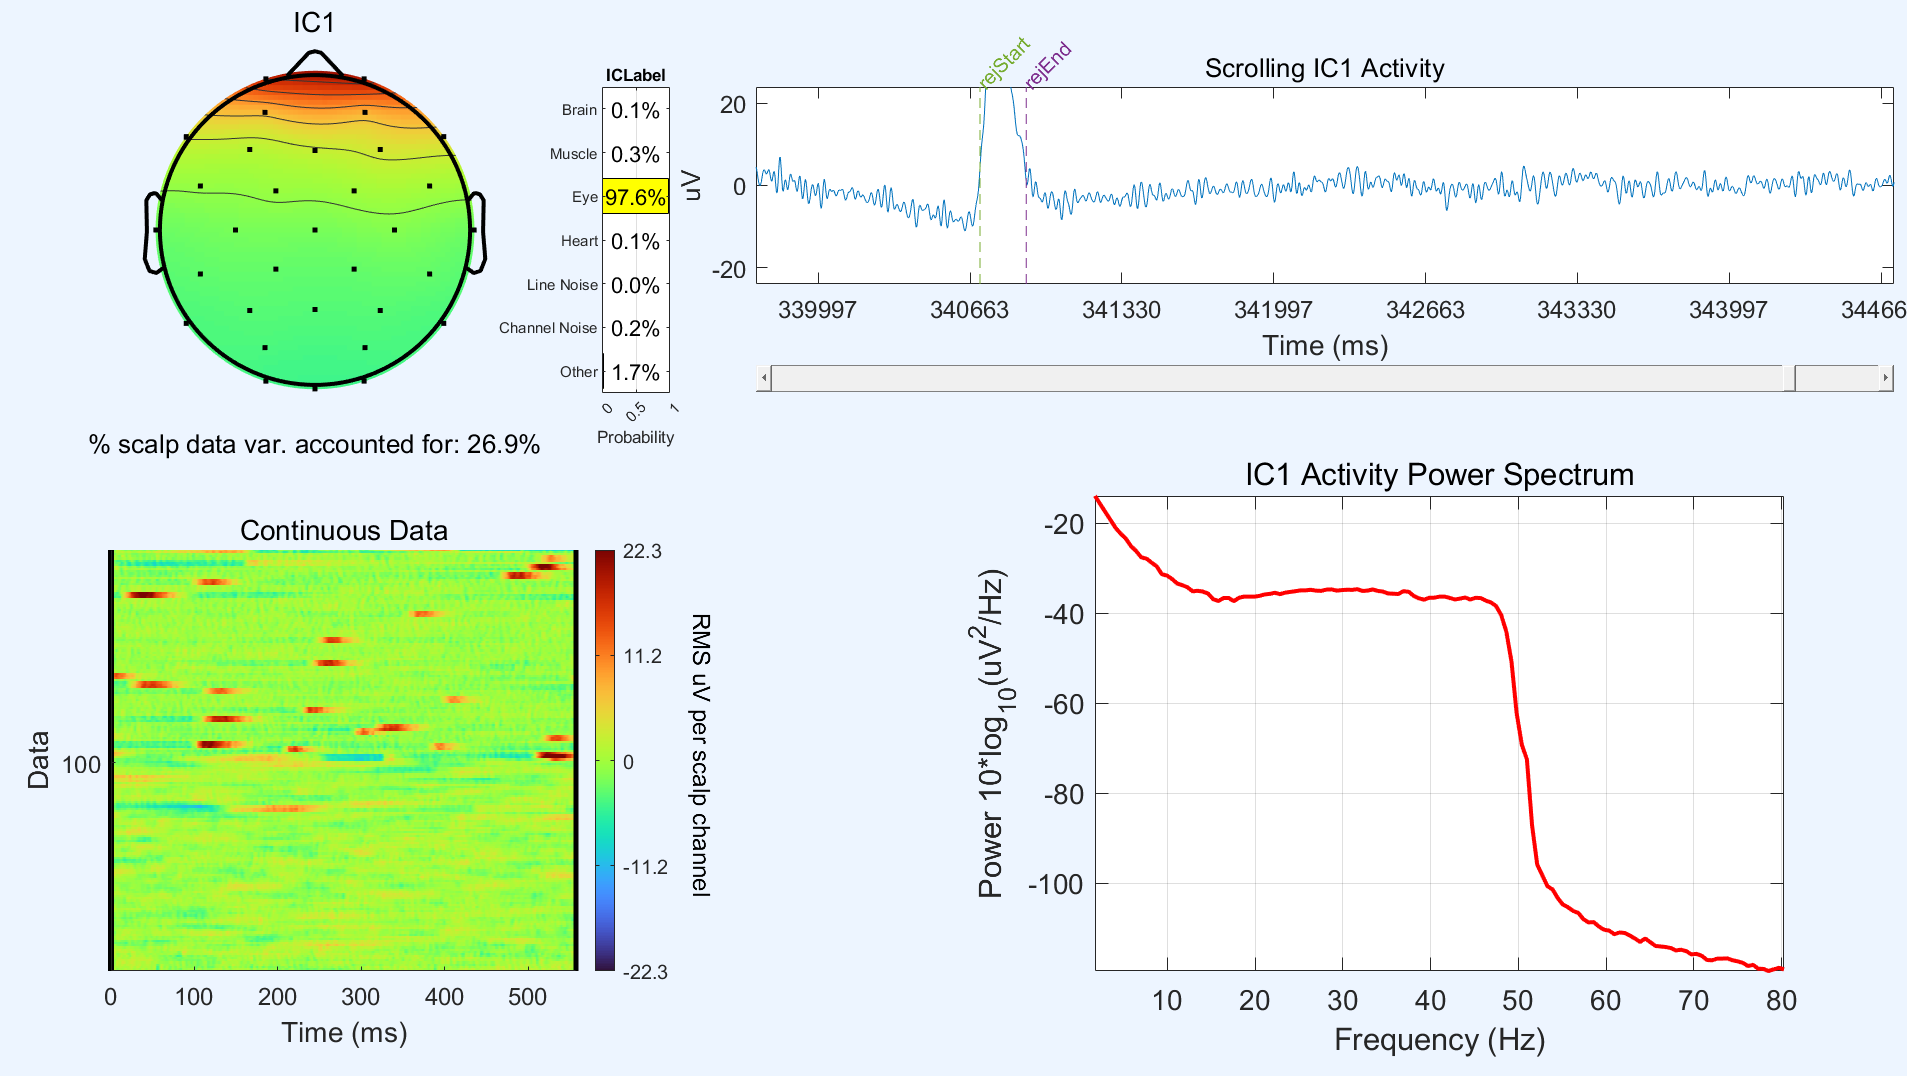
\includegraphics[width=1\linewidth]{./Chapter3_Methodology/Eye-blink via ICA label.png}
     \caption{Examples of components relevant with ocular artifacts.}
     \label{fig:ICA}
\end{figure}

Particularly, the application of ICA seems to be particularly useful in removing blinks and other oculomotor artifacts. Using ICA to correct artifacts is generally considered the best, since it does not assume orthogonal or gaussian behavior of the individual signals. 
In contrast, principal component analysis (PCA) assumes that all signals are orthogonal and creates a succession of orthogonal base vectors, where each vector will account for as much variance as possible. 
As a result, the first vector from PCA is significantly larger in magnitude than all the subsequent vectors. 
When the signal to noise ratio is low, important information in these subsequent vectors can get lost\cite{makkar2023}.

\section{Artifact detection using a neural network model}

For the model, we chose Temporal Convolutional Network (TCN) architecture. While sequence-to-sequence tasks are commonly solved with recurrent neural network architectures, as it was previously shown that convolutional neural networks can match the performance of recurrent networks on typical sequence modeling tasks or even outperform them.

We begin by describing our architecture for convolutional sequence prediction. The main building block of a TCN is a dilated causal convolution layer and it is based upon two principles: the fact that the network produces an output of the same length as the input, and the fact that there can be no leakage from the future into the past. To accomplish the first point, the TCN uses a 1D fully-convolutional network (FCN) architecture, where each hidden layer is the same length as the input layer, and zero padding of length (kernel size - 1) is added to keep subsequent layers the same length as previous ones. To achieve the second point, the TCN uses causal convolutions, convolutions where an output at time \(t\) is convolved only with elements from time \(t\) and earlier in the previous layer. In this context, "causal" means that the activations computed for a particular time step cannot depend on activations from future time steps.

A simple causal convolution is only able to look back at a history with size linear in the depth of the network. This makes it challenging to apply the aforementioned causal convolution on sequence tasks, especially those requiring longer history like in our case.

\begin{figure}[H]
    \centering
    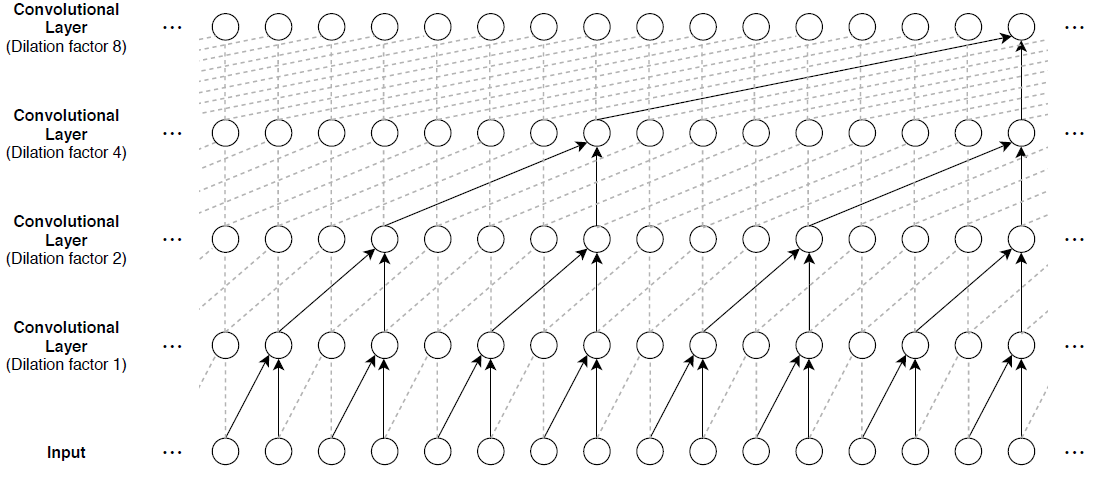
\includegraphics[width=1\linewidth]{images/Chapter3_Methodology/dilation factor.png}
    \caption{A dilated causal convolution with dilation factors d = 1, 2, 4, 8 and filter size k = 2.}
    \label{fig:dilation-factor}
\end{figure}

This gives us two ways to increase the receptive field of the TCN: choosing larger filter sizes \(k\) and increasing the dilation factor \(d\), where the effective history of one such layer is \((k - 1)d\). As is common when using dilated convolutions, we increase \(d\) exponentially with the depth of the network (i.e., \(d = O(2^i)\) at level \(i\) of the network). This ensures that there is some filter that hits each input within the effective history, while also allowing for an extremely large effective history using deep networks.

Our TCN model consists of multiple residual blocks, and a residual block contains a branch leading out to a series of transformations \(\mathcal{F}\), whose outputs are added to the input x of the block:
\begin{equation}
    o = Activation(x + \mathcal{F}(x))
    \label{eq:activation}
\end{equation}
where \(o\) is the output of the residual block and \(x\) is the input to the residual block.

This effectively allows layers to learn modifications to the identity mapping rather than the entire transformation, which has repeatedly been shown to benefit very deep networks.

The residual block for our TCN is shown in Figure \ref{fig:residual-block}, where each of the residual blocks contains two sets of dilated causal convolution layers with the same dilation factor, followed by normalization, ReLU activation, and spatial dropout layers. The network adds the input of each block to the output of the block (including a 1-by-1 convolution on the input when the number of channels between the input and output do not match) and applies a final activation function. 

\begin{figure}[H]
    \centering
    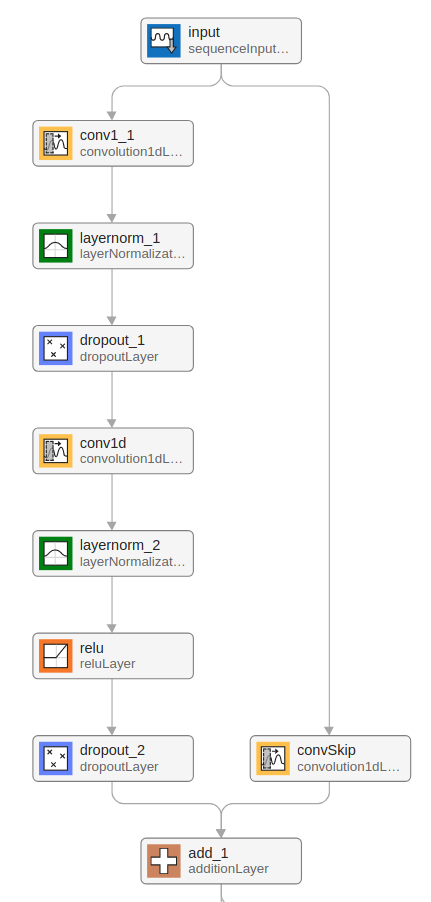
\includegraphics[width=0.5\linewidth]{images/Chapter3_Methodology/residual.png}
    \caption{TCN residual block. An 1-by-1 convolution is added when residual input and output have different dimensions.}
    \label{fig:residual-block}
\end{figure}

Lastly, in the Figure \ref{fig:tcn-model}. we present an overview of the whole model architecture which contains four residual blocks described above and shown in greater detail. After the residual blocks we end with fully-connected layer which maps the extracted features to the output space, and lastly we apply a softmax activation which produces a probability distribution over the predicted classes, in our case if it is an artifact (class 1) or not (class 0).

\begin{figure}[H]
    \centering
    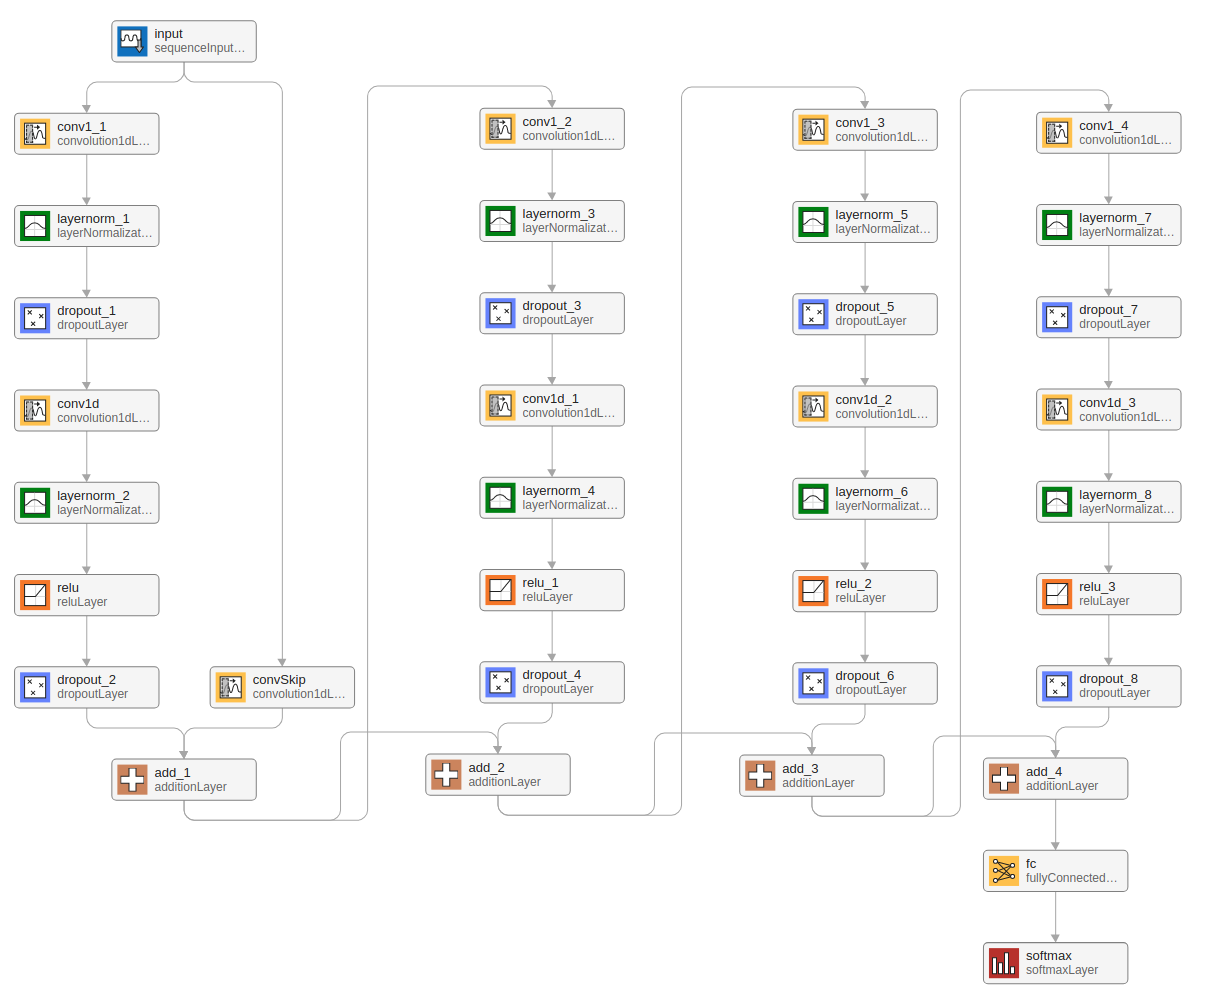
\includegraphics[width=1\linewidth]{images/Chapter3_Methodology/tcn-model.png}
    \caption{Architecture of our TCN model with four residual blocks.}
    \label{fig:tcn-model}
\end{figure}

%%%%%%%%%%%%%%%%%%%%%%%%%%%%%%%%%% Chapter 4: Results %%%%%%%%%%%%%%%%%%%%%%%%%%%%%%%%%%%%%

\chapter{Results}
\thispagestyle{fancy}

In this chapter, we report the performance of our model using key metrics such as accuracy, precision, and recall. These results show how well the model identifies and classifies artifacts in our test dataset.
We will examine the results of our thorough testing process. The outcomes of our model's tests, both qualitative and quantitative, are presented here in our analysis. In addition to highlighting the model's potential, this assessment points out the drawbacks or areas in need of more development.

The main training process was done on one dataset, with an already established model architecture without any modifications to its structure or hyperparameters. The focus of this training was replicating the performance suggested in previous studies, and using it to prove our hypothesis. As a result, no validation dataset was included in the training phase, and the choice was made based on lack of changes to the model that would require additional validation. 
Additionally, the model is trained and evaluated in a way where it is subject-invariant, so we ensure generalization across individuals. The identity of the subject or any subject specific features are not used as an input or conditioning factor, as we are only interested in eye-blink events.

Training was performed on the "raw-caffeine\_318" and "raw-caffeine\_366" subset of the dataset, while the later evaluation was performed on "raw-caffeine\_311" subset.

To validate our hypothesis, the model has been trained in supervised manner, where ICA-based label was used as the ground truth and to define target labels or segmentation boundaries representing artifact presence in our data. By aligning the training objective with ICA-based labels, we guide the model to mimick the ICA's ability to detect artifacts, and serve as a proof that CNN can approximate or even replicate traditional signal decomposition techniques in identifying noise in EEG data.

\section{Results of training}

In Fig. \ref{fig:training} we display the accuracy and loss training measures. The model was trained over 60 epochs with a base learning rate set to 0.001. Within the first few epochs, the model achieves nearly perfect training accuracy, indicating rapid convergence of the accuracy curve.
Also we can see this in the training loss curve, where we observe steep decline during the initial iterations and in the further training it stabilizes at minimal values.
This demonstrates the model's ability to successfully fit the training data and is consistent with our expectations of it.

\begin{figure}[H]
     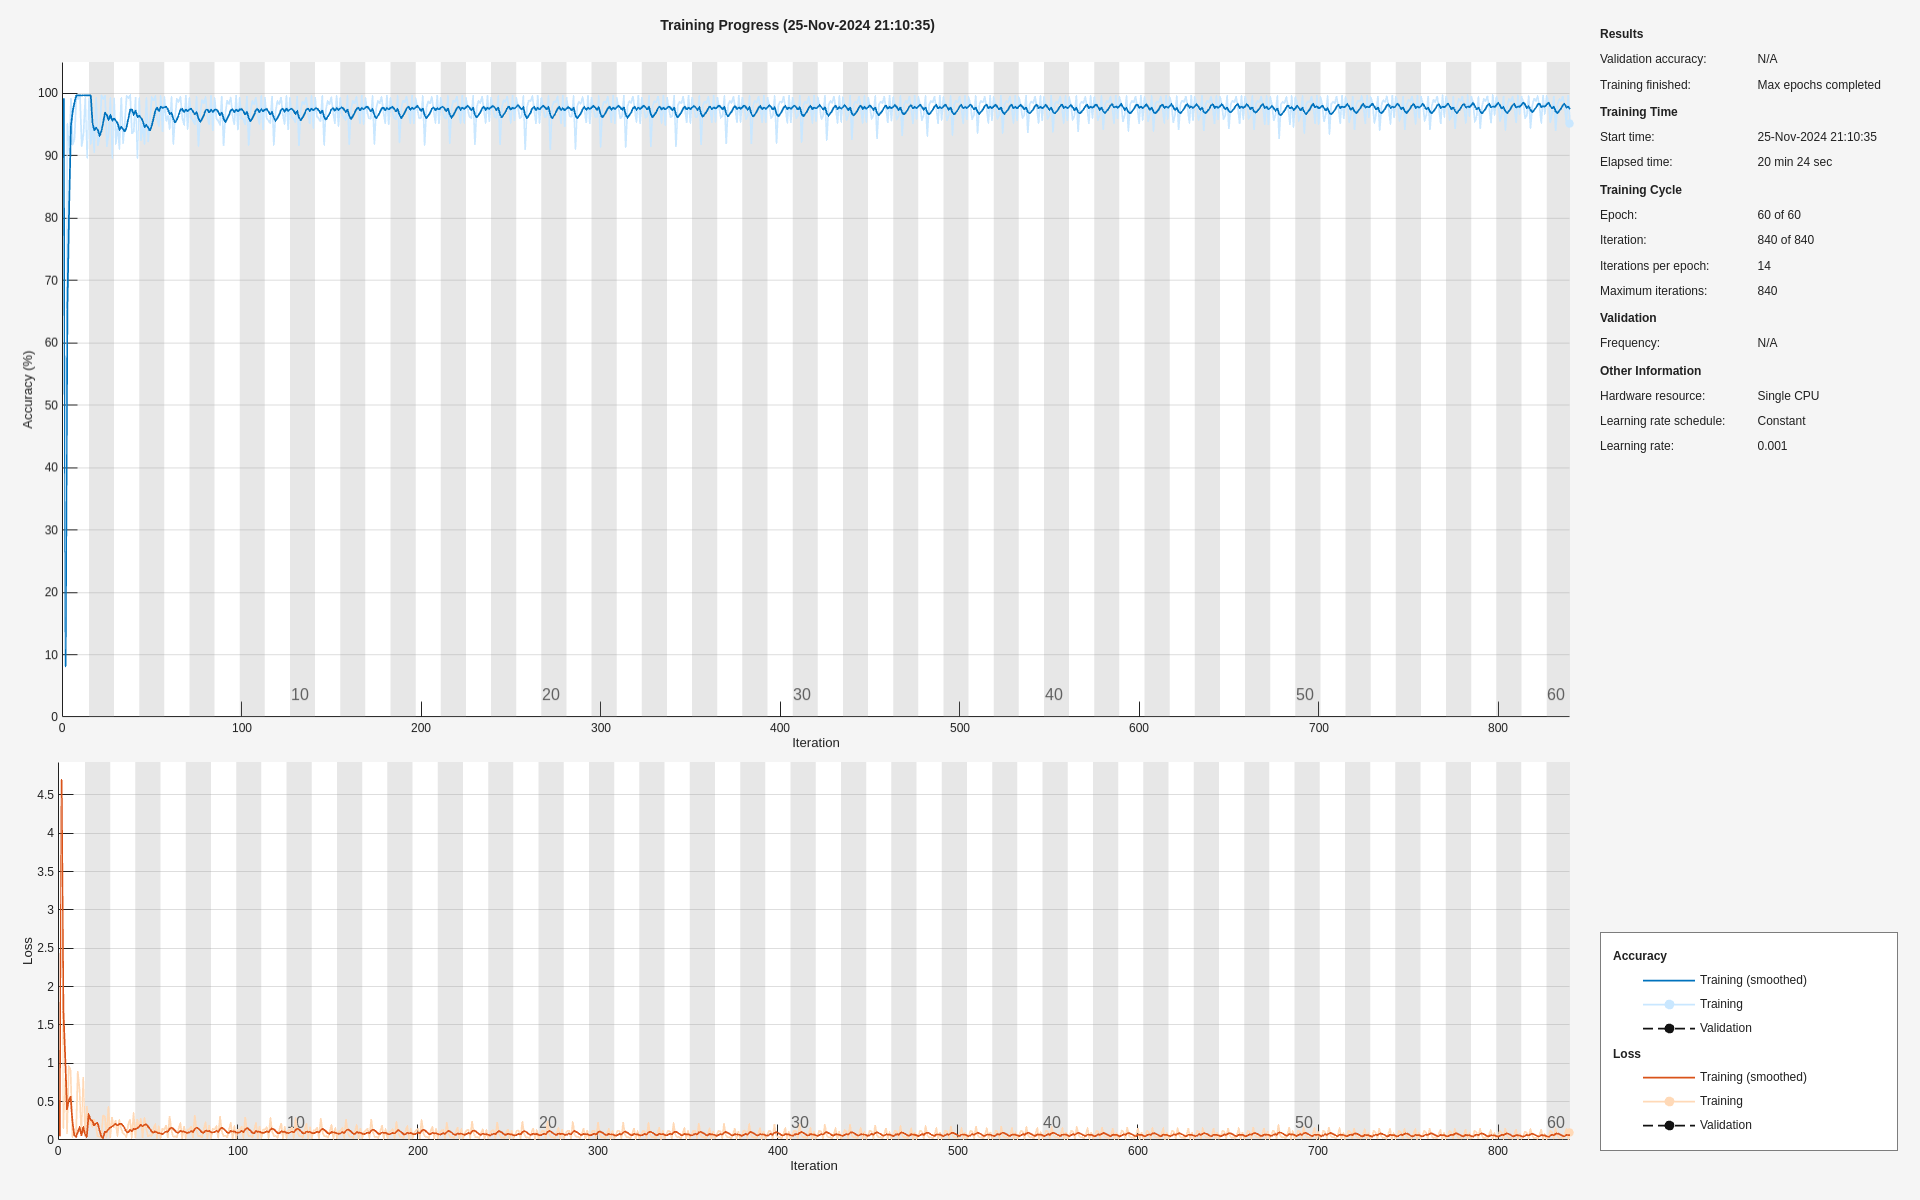
\includegraphics[width=1\linewidth]{./new_training/training_chart_new.png}
     \caption{Results of training}
     \label{fig:training}
\end{figure}

\section{Results of testing the model}

The confusion matrix, shown in Figure \ref{fig:confusion-matrix}, shows the performance of classification using the trained model. We can see the following:
\begin{itemize}
    \item True Negatives: 92288
    \item False Negatives: 134
    \item True Positives: 7012
    \item False Positives: 1598
\end{itemize}

Based on these results, we calculate the accuracy of the predictions per data points, which is approximately \(98.28\%\), with the precision of detecting positive data points being \(81.44\%\). 

\begin{figure}[H]
    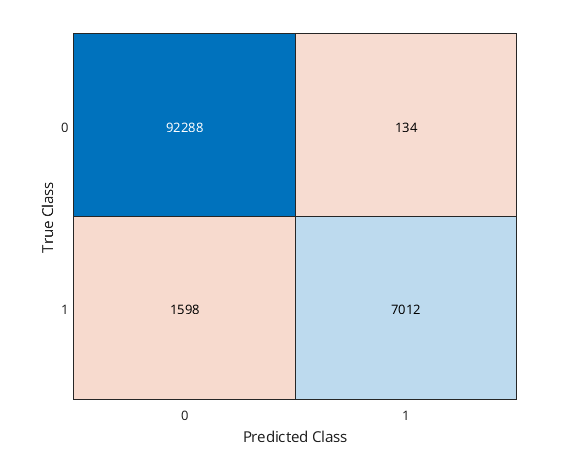
\includegraphics[width=1\linewidth]{./new_training/training_test_data_confusion_chart_new.png}
    \caption{Confusion matrix}
    \label{fig:confusion-matrix}
\end{figure}

These results indicate that the model maintained relatively high precision and accuracy during testing, suggesting that while false positives are rare, some artifacts can be missed. While this shows us the accuracy and precision of detecting if at some point we have a 0 or a 1 data point, it does not paint the full picture if the model correctly predicted an artifact or not, as artifacts segments expand over multiple data points. That is why the next thing we have to look at is artifact level evaluation, and how it performs when looking into segments rather than data points and this is visually demonstrated in the Figure \ref{fig:time-series} and fully covered in the next section.

\begin{figure}[H]
    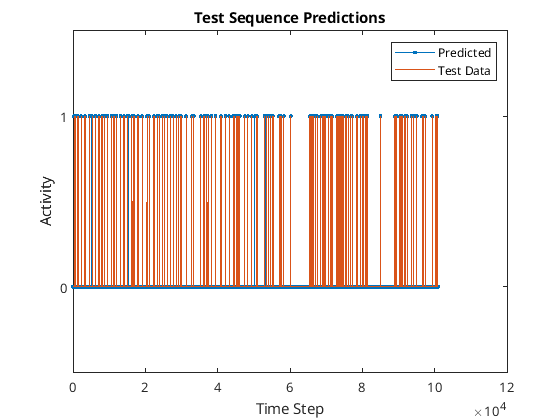
\includegraphics[width=1\linewidth]{./new_training/test_sequence_predictions_new.png}
    \caption{Time-series line chart}
    \label{fig:time-series}
\end{figure}

\section{Artifact based evaluation}

In the Table \ref{tab:artifact_eval}, we present a comparison between the number of ground-truth artifacts that were labeled by ICA, and the ones predicted by our model. In this case, an overlap refers to instances where a predicted artifact segment intersects with a ground-truth artifact segment. Important to note is that the overlap does not require exact alignment in terms of duration or start–end boundaries. As long as there is significant intersection between a predicted and true artifact, it is considered a correctly detected artifact.

\begin{table}[ht]
\centering
\resizebox{\textwidth}{!} & \textbf{Missed} & \textbf{False Positives} \\
\hline
2019.07.24\_11.51.14 & 34  & 66  & 30  & 88\%  & 4  & 36 \\
2019.07.24\_12.54.43 & 93  & 145 & 91  & 98\%  & 2  & 54 \\
2019.07.24\_11.53.06 & 29  & 46  & 28  & 97\%  & 1  & 18 \\
2019.07.24\_11.54.47 & 15  & 38  & 15  & 100\% & 0  & 23 \\
2019.07.24\_13.02.42 & 224 & 255 & 222 & 99\%  & 2  & 33 \\
2019.07.24\_12.04.44 & 65  & 89  & 61  & 94\%  & 4  & 28 \\
2019.07.24\_12.08.46 & 86  & 146 & 80  & 93\%  & 6  & 66 \\
2019.07.24\_12.13.23 & 109 & 128 & 108 & 99\%  & 1  & 20 \\
\hline
\end{tabular}%
}
\caption{Artifact Evaluation per Recording}
\label{tab:artifact_eval}
\end{table}

In the artifact-based results we can see a higher precision than we saw in data point precision, where detection rates for records range from 88\% to 100\%. We can also observe that besides one recording with accuracy of 88\%, all others are above 90\%,and this shows the model's strong ability to detect artifacts, almost identically to ICA-based ones that were used as ground truth in this comparison.

Despite the model's high prediction rate, we also can observe a notable amount of false positives, where sometimes in few recordings they even exceed the ground truth.

\newpage
\section{Alternative model comparison}

In this section we explore if the model that we used can be trained with changed hyperparameters to make it simpler without impacting the accuracy. Previously we observed the models performance when trained with four residual blocks, and here we will present simpler versions of the same model, and test its accuracy using: one residual block, two residual blocks, and three residual blocks.
We applied the same method of training and testing, using two subjects from the dataset for training and one for testing the predictions. Same as above we will use artifact-based evaluation on the same subject in the dataset to display the results.

\subsection{One residual block model}

The training accuracy of the same model with only one residual block was ~97.467\%.
From the Figure \ref{tab:artifact_eval_1_block}. we can see that while the model achieves consistently high detection rates, that is over \textgreater90\% for each recording, a substantial number of false positives appear, in one recording even over 300. This indicates that our model with reduced amount of residual blocks tends to overpredict artifacts and is not very suited for our use-case.

\begin{table}[htbp]
\centering
\resizebox{\textwidth}{!} & \textbf{Missed} & \textbf{False Positives} \\
\hline
2019.07.24\_11.51.14 & 34 & 168 & 31 & 91\% & 3 & 137 \\
2019.07.24\_12.54.43 & 93 & 203 & 91 & 98\% & 2 & 112 \\
2019.07.24\_11.53.06 & 29 & 58 & 28 & 97\% & 1 & 30 \\
2019.07.24\_11.54.47 & 15 & 73 & 15 & 100\% & 0 & 58 \\
2019.07.24\_13.02.42 & 224 & 319 & 222 & 99\% & 2 & 97 \\
2019.07.24\_12.04.44 & 65 & 178 & 63 & 97\% & 2 & 115 \\
2019.07.24\_12.08.46 & 86 & 440 & 82 & 95\% & 4 & 358 \\
2019.07.24\_12.13.23 & 109 & 158 & 109 & 100\% & 0 & 49 \\
\hline
\end{tabular}%
}
\caption{Artifact-level evaluation of model predictions with one residual block}
\label{tab:artifact_eval_1_block}
\end{table}


\subsection{Two residual blocks model}

The training accuracy of the same model with only one residual block was ~98.15\%, which is a slightly higher accuracy than the model with one residual block.
In Figure \ref{tab:artifact_eval_2_blocks}, we can still observe a high number of predicted artifacts, but also an interesting detection accuracy for one record with only 20\% of correct predictions. Based on this, this variation of the model performed the worst out of all of the four iterations, but the number of false positives dropped significantly by introducing more complexity with another residual block.

\begin{table}[htbp]
\centering
\resizebox{\textwidth}{!} & \textbf{Missed} & \textbf{False Positives} \\
\hline
2019.07.24\_11.51.14 & 34 & 150 & 31 & 91\% & 3 & 119 \\
2019.07.24\_12.54.43 & 93 & 234 & 91 & 98\% & 2 & 143 \\
2019.07.24\_11.53.06 & 29 & 81 & 28 & 97\% & 1 & 53 \\
2019.07.24\_11.54.47 & 15 & 80 & 15 & 100\% & 0 & 65 \\
2019.07.24\_13.02.42 & 224 & 306 & 223 & 100\% & 1 & 83 \\
2019.07.24\_12.04.44 & 65 & 173 & 60 & 92\% & 6 & 113 \\
2019.07.24\_12.08.46 & 86 & 288 & 81 & 94\% & 5 & 207 \\
2019.07.24\_12.13.23 & 109 & 288 & 22 & 20\% & 87 & 266 \\
\hline
\end{tabular}%
}
\caption{Artifact-level evaluation of model predictions with two residual blocks}
\label{tab:artifact_eval_2_blocks}
\end{table}

\subsection{Three residual blocks model}

The training accuracy of the same model with only one residual block was ~98.35\%.
Lastly, Figure \ref{tab:artifact_eval_3_blocks}. shows us similar picture to model with two residual blocks, where the number of predicted artifacts and false positives remains similar, and even in certain recordings exceeds the ones from two residual blocks model. By increasing more complexity to three, we sacrificed the previous simplicity we had with 2 residual blocks but we did not gain any significant performance from the model as we can see from both training accuracy which had slight increase and in arifact-level evaluation. 

\begin{table}[htbp]
\centering
\resizebox{\textwidth}{!} & \textbf{Missed} & \textbf{False Positives} \\
\hline
2019.07.24\_11.51.14 & 34 & 150 & 31 & 91\% & 3 & 119 \\
2019.07.24\_12.54.43 & 93 & 208 & 91 & 98\% & 2 & 117 \\
2019.07.24\_11.53.06 & 29 & 70 & 28 & 97\% & 1 & 42 \\
2019.07.24\_11.54.47 & 15 & 79 & 15 & 100\% & 0 & 64 \\
2019.07.24\_13.02.42 & 224 & 304 & 223 & 100\% & 1 & 81 \\
2019.07.24\_12.04.44 & 65 & 158 & 61 & 94\% & 4 & 97 \\
2019.07.24\_12.08.46 & 86 & 304 & 81 & 94\% & 5 & 223 \\
2019.07.24\_12.13.23 & 109 & 162 & 108 & 99\% & 1 & 54 \\
\hline
\end{tabular}%
}
\caption{Artifact-level evaluation of model predictions with three residual blocks}
\label{tab:artifact_eval_3_blocks}
\end{table}

\section{Discussion}

The results of our study indicate that the proposed model, trained on our data is highly capable of detecting eye-blink artifacts in EEG recordings. We also made sure that the model is trained on relevant artifacts, that were made by ICA and used as a ground truth of this research. The results show high detection rates across all recordings, with most of them exceeding 90\%, and this number refers to overlaps between the predicted artifacts and ground truth artifacts. In addition, we saw that some recordings had all ground truth artifacts detected correctly, reaching detection rate of 100\%.

Applying ICA-based EEG imaging to studies involving multiple subjects and/or sessions requires a method for combining IC source location and activity measure information for ICs decomposed from multiple data sets.\cite{bigdely2013measure} As a result we have chosen the overlap-based matching deliberately, as artifact boundaries in EEG data can be ambiguous, and these can often vary both with ICA-based labeling and by manual expert annotations. That is the main reason to focus on temporal overlap rather than data points comparisson, as this allows us to rate the precision of the model based on it ability to predict artifacts, that is the presence of artifact rather than its exact segment boundaries. With this we highlight more the practical use that would happen in preprocessing, where the focus is on artifact removal not exact data points. An example of segments not exactly overlapping can be seen in the Figure \ref{fig:overlaps} where rejStart and rejEnd are created by ICA, where rejStart-new and rejEnd-new are created by our model.

\begin{figure}[H]
     \centering
     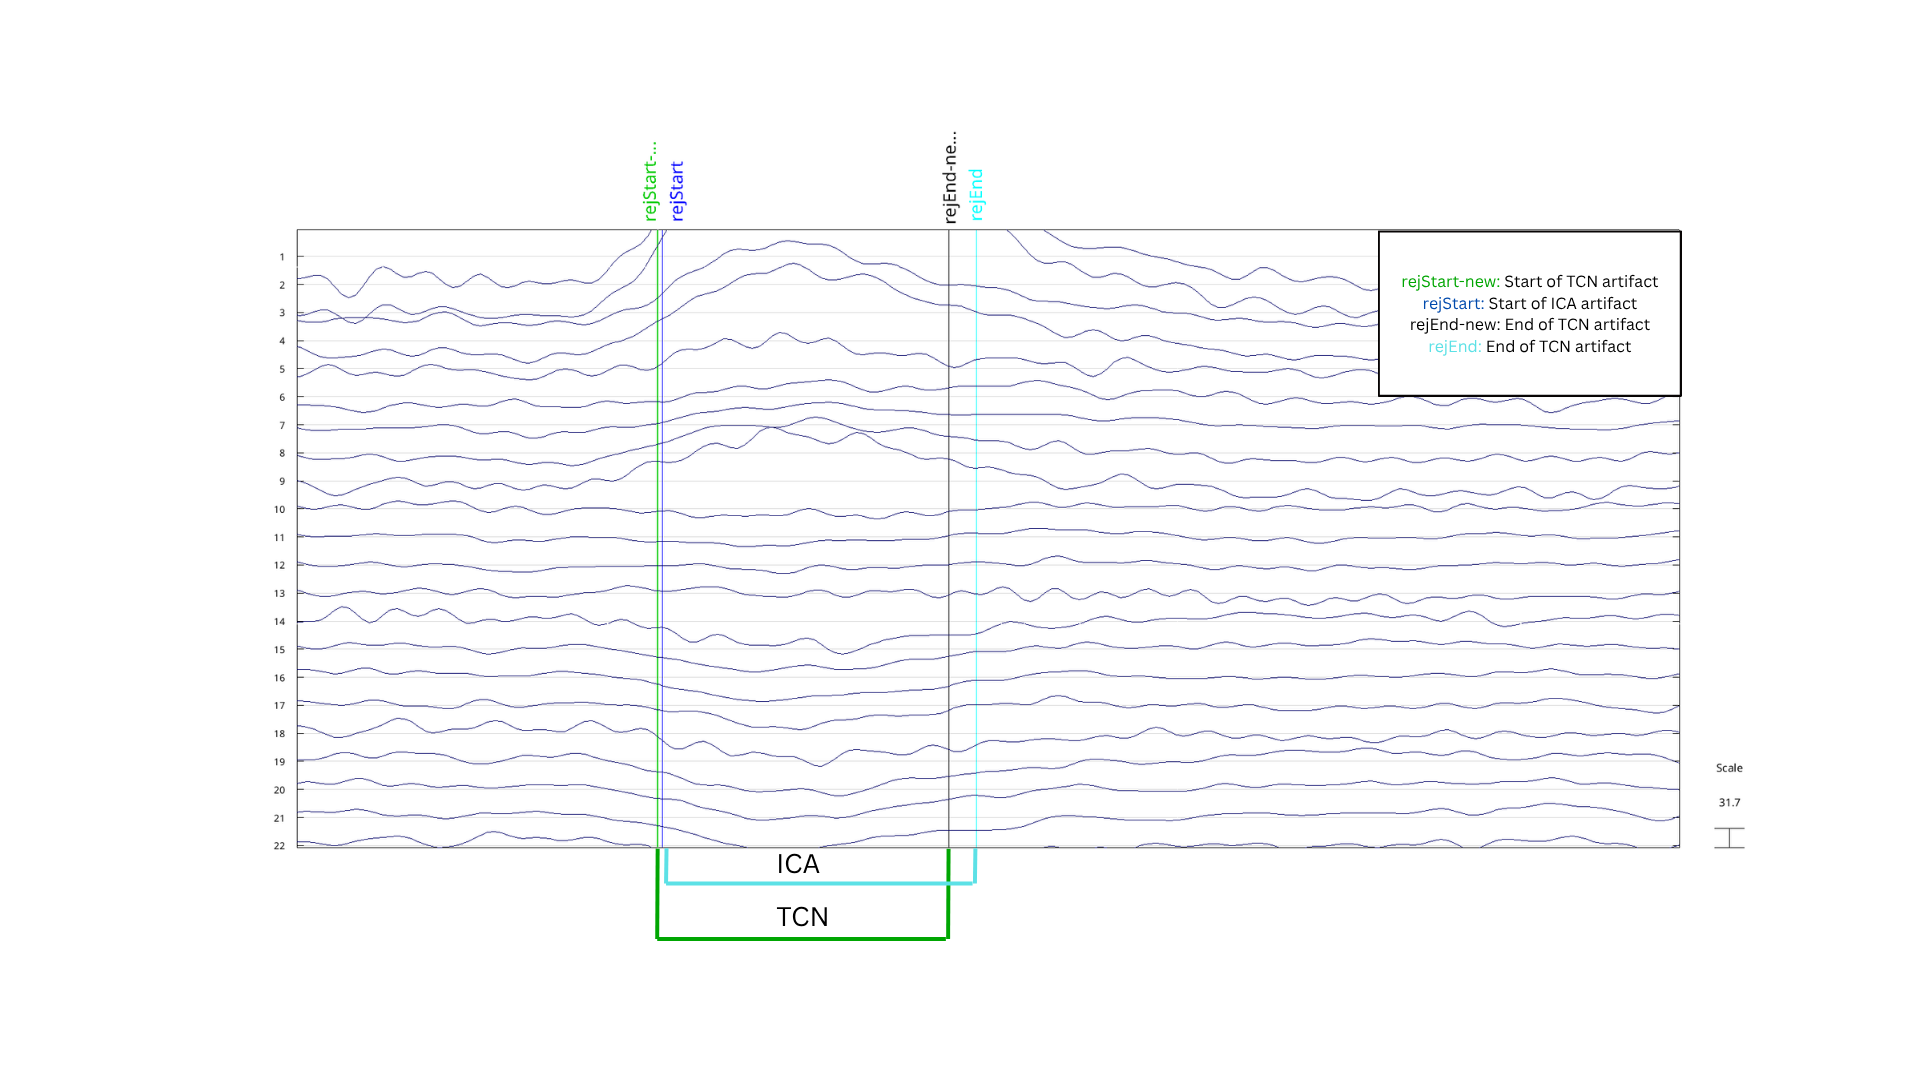
\includegraphics[width=1\linewidth]{./misc/artifact-overlaps.png}
     \caption{ICA-label based artifacts overlapping with TCN model-based artifacts}
     \label{fig:overlaps}
\end{figure}

Although the detection rates were consistently high, our model did produce a substantial number of false positives in for most recordings when comparing to ICA-based labels. This likely stems from the models learning, preferring to label noisy segments as artifacts rather than missing an artifact. While this reduces our models precision, from practical standpoint it is easier to deal with by manually reviewing, than missing artifacts and distorting the analysis or classification of EEG data. Additionally, what we saw is that certain artifacts have very small segments, sometimes just before the actual artifact or just after the ICA-based artifact segment has ended.

From generalization perspective, our model performed well on new, previously unseen EEG recordings, showing that it did not overfit to recording specific features. However, for future studies it would be great to see how our model compares to artifacts that were manually annotated by an expert in the field, even though this would likely show similar variance in segment boundaries.

%%%%%%%%%%%%%%%%%%%%%%%%%%%%%%%%%% Chapter 5: Discussion and conclusion %%%%%%%%%%%%%%%%%%%%%%%%%%%%%%%%%%%%%


\chapter{Conclusion}
\thispagestyle{fancy}

This thesis is motivated by goal of finding if the proposed model could be trained to detect specific events in EEG data, that would also be invariant to inter- and intra-subject differences and to inherent noise associated with EEG data. We propose a novel methodology for learning representations from multi-channel EEG time-series, and demonstrate its advantages and disadvantages against already established tool (ICA). The proposed approach demonstrates similar results to the state-of-the-art results in detecting eye-blink artifacts. The approach we used proved that the model can be trained to detect eye-blink artifacts, with similar accuracy to ICA.
As a future direction, it would be possible to use unsupervised pretraining methods with larger unlabeled EEG datasets to train the network to detect other signals in EEG data, not just eye-blink artifacts.


%%%%%%%%%%%%%%%%%%%%%%%%%%%%%%%%%% Chapter 6: Literature %%%%%%%%%%%%%%%%%%%%%%%%%%%%%%%%%%%%%

\begin{thebibliography}{99}
\thispagestyle{fancy}

\bibitem{wikipediaEEG}
     "Electroencephalography." \emph{Wikipedia, The Free Encyclopedia}. 
     Last modified May 23, 2025. Available at: \url{https://en.wikipedia.org/wiki/Electroencephalography}. Accessed May 24, 2025.

\bibitem{teplan2002}
     Teplan, Michal. 
     \emph{"Fundamentals of EEG Measurement."} 
     Published in *Measurement Science Review*, vol. 2, 2002. Available at: \url{https://www.researchgate.net/publication/228599963_Fundamental_of_EEG_Measurement}.

\bibitem{khalifa2012}
     Khalifa, Wael, Abdel-Badeeh M. Salem, Kenneth Revett, and Mohamed Roushdy.  
     \emph{"A Survey of EEG Based User Authentication Schemes."} 
     Presented at a conference in May 2012. Available at: \url{https://www.researchgate.net/publication/257449958_A_Survey_of_EEG_Based_User_Authentication_Schemes}.

\bibitem{wikipedia1020}
    "10--20 System (EEG)." \emph{Wikipedia, The Free Encyclopedia}. Last modified July 2024. Available at: \url{https://en.wikipedia.org/wiki/10-20_system_(EEG)}. Accessed May 24, 2025.
     
\bibitem{nunez2016}
     Michael Nunez, Paul Nunez, and Ramesh Srinivasan, 
     \emph{Electroencephalography (EEG): Neurophysics, Experimental Methods, and Signal Processing}, 
     Jan. 1, 2016, pp. 175--197, ISBN: 978-1-4822-2097-1, DOI: \url{https://doi.org/10.13140/RG.2.2.12706.63687}.

\bibitem{bai2018}
     Bai, Shaojie, J. Zico Kolter, and Vladlen Koltun. 
     \emph{"An Empirical Evaluation of Generic Convolutional and Recurrent Networks for Sequence Modeling."} 
     Preprint, submitted April 19, 2018. Available at: \url{https://arxiv.org/abs/1803.01271}.
     
\bibitem{makkar2023}
     Makkar, Krish, Bisen, Anvikshaa, and Ijmtst, Editor, 
     \emph{EEG Signal Processing and Feature Extraction}, 
     International Journal for Modern Trends in Science and Technology, vol. 9, pp. 45--50, 2023, 
     DOI: \url{https://doi.org/10.1007/978-981-13-9113-2}.   

\bibitem{Lesar2025}
    Lesar, M., Sajovic, J., Novaković, D., Primožič, M., Vetrih, E., Sajovic, M., Žnidaršič, A., Rogelj, P., Daffertshofer, A., Levnajić, Z., and Drevenšek, G.
    \newblock The complexity of caffeine's effects on regular coffee consumers.
    \newblock \emph{Heliyon}, 11(2), 2025.
    \newblock Elsevier.
    \newblock \url{https://doi.org/10.1016/j.heliyon.2024.e41471}.

\bibitem{islam2023}
     Islam, Mohammad K., and Arash Rastegarnia. 
     \emph{"Recent Advances in EEG (Non-Invasive) Based BCI Applications."} 
     Published in *Frontiers in Computational Neuroscience*, vol. 17, 2023. Available at: \url{https://doi.org/10.3389/fncom.2023.1151852}.

\bibitem{lesar2025}
     Lesar, Mateja, Jakob Sajovic, Dušanka Novaković, Maša Primožič, Eva Vetrih, Martin Sajovic, Anja Žnidaršič, Peter Rogelj, Andreas Daffertshofer, Zoran Levnajić, and Gorazd Drevenšek.  
     \emph{"The Complexity of Caffeine's Effects on Regular Coffee Consumers."}  
     Published in *Heliyon*, vol. 11, no. 2, Elsevier, 2025. Available at: \url{https://doi.org/10.1016/j.heliyon.2024.e41471}.

\bibitem{bigdely2013measure}
    Bigdely-Shamlo, N., Mullen, T., Kreutz-Delgado, K., and Makeig, S. (2013).
    Measure projection analysis: A probabilistic approach to EEG source comparison and multi-subject inference.
    \textit{NeuroImage}, \textbf{72}, 287--303.
    \url{https://www.ncbi.nlm.nih.gov/pmc/articles/PMC4082972/}
    
    
     
     % There has to be an empty line here so that the page numbers of citations are properly displayed.
\end{thebibliography}
\newpage

%%%%%%%%%%%%%%%%%%%%%%%%%%%%%%%%%% Summary of the final project paper in Slovene  %%%%%%%%%%%%%%%%%%%%%%%%%%%%%%%%%%%%%

\chapter{Povzetek naloge v slovenskem jeziku}
\thispagestyle{fancy}

This chapter contains a longer summary of the final project paper in Slovene,
in total length between $4.000$ and $10.000$ characters (spaces included).


\addtocontents{toc}{\setcounter{tocdepth}{2}}
\end{document}